\documentclass[12pt]{article}

\usepackage[utf8]{inputenc}
\usepackage{amsmath}
\usepackage{amssymb}
\usepackage{graphicx}
\usepackage{booktabs}
\usepackage{algorithm}
\usepackage{algpseudocode}
\usepackage{hyperref}
\usepackage[margin=1in]{geometry}
\usepackage{float}

\title{Care Phenotype Analysis: A Mathematical Framework for Healthcare Pattern Recognition}
\author{Care Phenotype Analyzer Research Team}
\date{\today}

\begin{document}

\maketitle

\begin{abstract}
This document presents a comprehensive explanation of the mathematical principles underpinning the care phenotype analyzer framework. The care phenotype approach enables the identification of patient subgroups based on observable healthcare delivery patterns, which can reveal important variations in care practices that may not be explained by clinical factors alone. We demonstrate a methodological framework that employs unsupervised learning, statistical modeling, and fairness evaluation to analyze healthcare data patterns. Specifically, we explore k-means clustering for phenotype identification, statistical measures for quantifying unexplained variation, and mathematical formulations for evaluating fairness across demographic groups. This approach allows clinicians and researchers to identify potential disparities in healthcare delivery while accounting for legitimate clinical factors, providing a robust framework for understanding systematic patterns in healthcare data collection.
\end{abstract}

\section{Introduction}

Healthcare data collection patterns often exhibit significant variations that cannot be fully explained by clinical necessity. These variations may reflect both legitimate clinical differences and subjective decisions by medical staff. The identification and analysis of these patterns are crucial for understanding potential biases in healthcare datasets and developing more robust healthcare algorithms.

The concept of "care phenotypes" provides an objective framework for analyzing these patterns. Unlike traditional demographic-based approaches to evaluating healthcare disparities, care phenotypes focus on observable patterns in how patients are monitored and treated, providing a more direct measure of potential disparities in care delivery.

\subsection{Objectives}

The main objectives of this analytical framework are to:

\begin{itemize}
    \item Identify distinct care phenotypes through unsupervised learning
    \item Quantify the extent to which clinical factors explain observed variations
    \item Measure unexplained variation that may indicate potential biases
    \item Evaluate fairness across demographic groups using mathematically rigorous metrics
\end{itemize}

\section{Mathematical Framework}

\subsection{Data Representation}

We represent healthcare data as a matrix $X \in \mathbb{R}^{n \times m}$, where $n$ is the number of patients and $m$ is the number of features. These features include:

\begin{itemize}
    \item Clinical factors $C \in \mathbb{R}^{n \times p}$ (e.g., SOFA scores, Charlson comorbidity indices)
    \item Care patterns $P \in \mathbb{R}^{n \times q}$ (e.g., lab test frequencies, monitoring intervals)
    \item Demographic factors $D \in \mathbb{R}^{n \times r}$ (e.g., age, gender, ethnicity)
\end{itemize}

where $p + q + r = m$.

\subsection{Phenotype Creation via Clustering}

We employ k-means clustering to identify distinct care phenotypes based on observable care patterns. The mathematical formulation of the k-means algorithm is:

\begin{align}
\underset{\mathbf{S}}{\text{minimize}} \sum_{i=1}^{k} \sum_{\mathbf{x} \in S_i} \|\mathbf{x} - \boldsymbol{\mu}_i\|^2
\end{align}

where:
\begin{itemize}
    \item $k$ is the number of clusters (care phenotypes)
    \item $S = \{S_1, S_2, \ldots, S_k\}$ represents the set of clusters
    \item $\mathbf{x}$ is a data point in the feature space
    \item $\boldsymbol{\mu}_i$ is the centroid of cluster $S_i$
\end{itemize}

This clustering is performed after standardizing the features using z-score normalization:

\begin{align}
z_i = \frac{x_i - \mu}{\sigma}
\end{align}

where $\mu$ is the mean and $\sigma$ is the standard deviation of the feature.

\subsection{Unexplained Variation Analysis}

To separate legitimate clinical variation from potentially problematic unexplained variation, we employ a regression-based approach. For each care pattern $p$, we fit a linear regression model with clinical factors as predictors:

\begin{align}
p = \beta_0 + \sum_{i=1}^{j} \beta_i c_i + \epsilon
\end{align}

where:
\begin{itemize}
    \item $\beta_0$ is the intercept
    \item $\beta_i$ are the coefficients for clinical factors $c_i$
    \item $\epsilon$ is the error term (unexplained variation)
\end{itemize}

The total variation is decomposed as:

\begin{align}
\text{Total Variation} &= \text{Explained Variation} + \text{Unexplained Variation}\\
\text{Var}(p) &= \text{Var}(\hat{p}) + \text{Var}(\epsilon)
\end{align}

The coefficient of determination ($R^2$) quantifies the proportion of variation explained by clinical factors:

\begin{align}
R^2 = 1 - \frac{\sum_i (p_i - \hat{p}_i)^2}{\sum_i (p_i - \bar{p})^2}
\end{align}

\subsection{Statistical Significance of Phenotype Separation}

To assess whether the identified phenotypes represent statistically significant patterns, we employ analysis of variance (ANOVA). For each clinical factor $c$ and phenotype grouping $S$, we calculate:

\begin{align}
F = \frac{\text{Between-group variability}}{\text{Within-group variability}} = \frac{\sum_{i=1}^{k} n_i(\bar{c}_i - \bar{c})^2 / (k-1)}{\sum_{i=1}^{k}\sum_{j=1}^{n_i} (c_{ij} - \bar{c}_i)^2 / (n-k)}
\end{align}

where:
\begin{itemize}
    \item $k$ is the number of phenotypes
    \item $n_i$ is the number of patients in phenotype $i$
    \item $\bar{c}_i$ is the mean of clinical factor $c$ in phenotype $i$
    \item $\bar{c}$ is the overall mean of clinical factor $c$
    \item $n$ is the total number of patients
\end{itemize}

The p-value associated with this F-statistic quantifies the statistical significance of the separation.

\section{Fairness Evaluation Framework}

\subsection{Demographic Parity}

Demographic parity measures whether the rate of a particular prediction is the same across different demographic groups. Mathematically, for demographic groups $A$ and $B$:

\begin{align}
\text{Demographic Parity} &\iff P(\hat{Y}=1|A) = P(\hat{Y}=1|B)\\
\text{Disparity} &= |P(\hat{Y}=1|A) - P(\hat{Y}=1|B)|
\end{align}

where $\hat{Y}$ represents the model's predictions.

\subsection{Equal Opportunity}

Equal opportunity measures whether the true positive rate is the same across different demographic groups. Mathematically:

\begin{align}
\text{Equal Opportunity} &\iff P(\hat{Y}=1|Y=1,A) = P(\hat{Y}=1|Y=1,B)\\
\text{Disparity} &= |P(\hat{Y}=1|Y=1,A) - P(\hat{Y}=1|Y=1,B)|
\end{align}

where $Y$ represents the true labels.

\subsection{Care Pattern Disparity}

Care pattern disparity quantifies differences in observable care patterns across phenotypes. For a care pattern $p$ and phenotypes $i$ and $j$:

\begin{align}
\text{Care Pattern Disparity}_{i,j} = |\bar{p}_i - \bar{p}_j|
\end{align}

where $\bar{p}_i$ is the mean value of care pattern $p$ for patients in phenotype $i$.

\section{Implementation and Algorithm}

The implementation of this mathematical framework follows the algorithm below:

\begin{algorithm}[H]
\caption{Care Phenotype Analysis}
\begin{algorithmic}[1]
\State \textbf{Input:} Patient data $X$ with clinical factors $C$, care patterns $P$, and demographic factors $D$
\State \textbf{Output:} Phenotype labels, unexplained variation, fairness metrics

\Procedure{PhenotypeCreation}{$X, C, P$}
    \State Standardize care patterns $P$ using z-score normalization
    \State Apply k-means clustering to identify phenotype labels $L$
    \State Evaluate statistical significance of separation using ANOVA
    \State \Return phenotype labels $L$
\EndProcedure

\Procedure{UnexplainedVariation}{$X, C, P, L$}
    \For{each care pattern $p \in P$}
        \State Fit linear regression: $p = \beta_0 + \sum_{i} \beta_i c_i + \epsilon$
        \State Calculate explained variation: $\text{Var}(\hat{p})$
        \State Calculate unexplained variation: $\text{Var}(\epsilon)$
        \State Calculate $R^2$ and statistical significance
    \EndFor
    \State \Return unexplained variation metrics
\EndProcedure

\Procedure{FairnessEvaluation}{$X, D, L, \hat{Y}, Y$}
    \For{each demographic factor $d \in D$}
        \State Calculate demographic parity disparity
        \State Calculate equal opportunity disparity
    \EndFor
    \State Calculate care pattern disparities across phenotypes
    \State \Return fairness metrics
\EndProcedure
\end{algorithmic}
\end{algorithm}

\section{Results Interpretation}

\subsection{Phenotype Identification}

The k-means clustering identifies distinct patient subgroups (phenotypes) based on observable care patterns. These phenotypes represent different "care signatures" that patients receive, which may be influenced by both clinical factors and other systemic factors.

In the example implementation, we identify three distinct phenotypes:
\begin{itemize}
    \item Phenotype 0: Lower monitoring frequency (approximately 39\% of patients)
    \item Phenotype 1: Highest monitoring frequency (approximately 30\% of patients)
    \item Phenotype 2: Moderate monitoring frequency (approximately 31\% of patients)
\end{itemize}

\subsection{Unexplained Variation}

The unexplained variation analysis quantifies how much of the observed variation in care patterns cannot be explained by clinical factors. This unexplained variation may indicate potential biases or systemic factors influencing care delivery.

In our example, the coefficient of determination ($R^2$) for lab test frequency is approximately 0.61, indicating that about 61\% of the variation can be explained by clinical factors (SOFA and Charlson scores), while 39\% remains unexplained.

\subsection{Fairness Metrics}

The fairness evaluation reveals potential disparities across demographic groups:

\begin{itemize}
    \item Gender disparity in demographic parity: 0.064
    \item Ethnicity disparity in demographic parity: 0.084
    \item Age disparity in demographic parity: 0.578
\end{itemize}

These metrics indicate the degree to which predictions or care patterns differ across demographic groups, with higher values suggesting greater disparity.

\section{Visualization and Interpretation}

\subsection{Boxplot Analysis}

The boxplot visualization of lab test frequency by phenotype (Figure 1) allows for a visual comparison of the distribution of monitoring intensity across different phenotypes.

\begin{figure}[h]
\centering
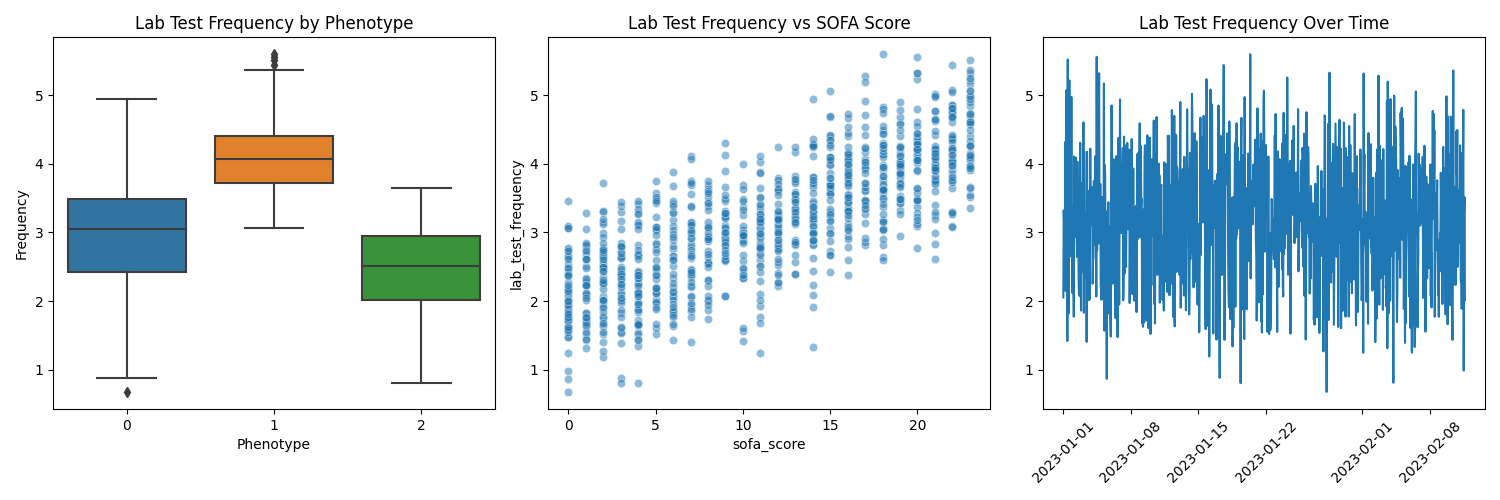
\includegraphics[width=0.8\textwidth]{../lab_test_analysis.png}
\caption{Left: Lab test frequency by phenotype. Middle: Lab test frequency vs. SOFA score. Right: Lab test frequency over time.}
\end{figure}

\subsection{Correlation Analysis}

The scatter plot of lab test frequency versus SOFA score visualizes the relationship between illness severity and monitoring intensity. The positive correlation observed aligns with clinical expectations that sicker patients receive more frequent monitoring.

\subsection{Temporal Analysis}

The time series plot of lab test frequency reveals temporal patterns in monitoring intensity, which may indicate systematic variations in care delivery over time.

\section{Discussion}

\subsection{Clinical Implications}

The identification of care phenotypes and quantification of unexplained variation have several important clinical implications:

\begin{itemize}
    \item Revealing potential biases in healthcare delivery that may not be apparent through traditional analyses
    \item Providing objective measures for quality improvement initiatives
    \item Supporting more equitable allocation of healthcare resources
    \item Informing the development of clinical decision support systems that account for potential biases
\end{itemize}

\subsection{Methodological Considerations}

Several methodological considerations are important for robust care phenotype analysis:

\begin{itemize}
    \item Selection of appropriate clinical factors to account for legitimate variation
    \item Determination of optimal cluster number for phenotype identification
    \item Choice of fairness metrics relevant to the specific healthcare context
    \item Interpretation of unexplained variation in the context of healthcare delivery
\end{itemize}

\section{Conclusion}

The care phenotype analysis framework provides a mathematically rigorous approach to understanding variations in healthcare delivery patterns. By separating legitimate clinical variation from unexplained variation and evaluating fairness across demographic groups, this framework enables researchers and clinicians to identify potential biases in healthcare delivery.

The implementation demonstrated in the lab\_test\_analysis\_example.py script illustrates the application of this framework to synthetic healthcare data, showcasing its potential for real-world healthcare data analysis. By focusing on observable care patterns rather than traditional demographic labels, this approach offers a novel and objective method for evaluating healthcare disparities.

\section{Future Directions}

Future development of this framework could include:

\begin{itemize}
    \item Integration of more sophisticated machine learning techniques for phenotype identification
    \item Development of causal inference methods to better understand the factors influencing care delivery
    \item Extension to longitudinal data analysis to capture temporal dynamics in care patterns
    \item Application to large-scale real-world healthcare datasets to validate the approach
\end{itemize}

\section{Appendix: Mathematical Foundations}

\subsection{K-means Clustering}

K-means clustering is an iterative algorithm that alternates between two steps:

\begin{enumerate}
    \item Assignment step: Assign each data point to the cluster with the nearest centroid
    \begin{align}
    S_i^{(t)} = \{\mathbf{x}_j : \|\mathbf{x}_j - \boldsymbol{\mu}_i^{(t)}\|^2 \leq \|\mathbf{x}_j - \boldsymbol{\mu}_{i'}^{(t)}\|^2 \; \forall \, i' = 1,\ldots,k\}
    \end{align}
    
    \item Update step: Calculate new centroids as the mean of all points in each cluster
    \begin{align}
    \boldsymbol{\mu}_i^{(t+1)} = \frac{1}{|S_i^{(t)}|} \sum_{\mathbf{x}_j \in S_i^{(t)}} \mathbf{x}_j
    \end{align}
\end{enumerate}

The algorithm converges when the assignments no longer change.

\subsection{Linear Regression}

Linear regression estimates the relationship between predictors $X$ and response $y$ by minimizing the sum of squared residuals:

\begin{align}
\hat{\boldsymbol{\beta}} = \underset{\boldsymbol{\beta}}{\text{argmin}} \sum_{i=1}^{n} (y_i - \mathbf{x}_i^T \boldsymbol{\beta})^2 = (X^T X)^{-1} X^T y
\end{align}

The coefficient of determination ($R^2$) is calculated as:

\begin{align}
R^2 = 1 - \frac{SS_{res}}{SS_{tot}} = 1 - \frac{\sum_i (y_i - \hat{y}_i)^2}{\sum_i (y_i - \bar{y})^2}
\end{align}

\subsection{Analysis of Variance (ANOVA)}

One-way ANOVA tests the null hypothesis that samples from different groups are drawn from populations with the same mean. The F-statistic is:

\begin{align}
F = \frac{MS_{between}}{MS_{within}} = \frac{\sum_{i=1}^{k} n_i(\bar{x}_i - \bar{x})^2 / (k-1)}{\sum_{i=1}^{k}\sum_{j=1}^{n_i} (x_{ij} - \bar{x}_i)^2 / (n-k)}
\end{align}

Under the null hypothesis, this statistic follows an F-distribution with $(k-1, n-k)$ degrees of freedom.

\end{document}
